\documentclass{ximera}
%% You can put user macros here
%% However, you cannot make new environments

\listfiles

\graphicspath{
{./}
{./LTR-0070/}
{./VEC-0060/}
{./APP-0020/}
}

\usepackage{tikz}
\usepackage{tkz-euclide}
\usepackage{tikz-3dplot}
\usepackage{tikz-cd}
\usetikzlibrary{shapes.geometric}
\usetikzlibrary{arrows}
%\usetkzobj{all}
\pgfplotsset{compat=1.13} % prevents compile error.

%\renewcommand{\vec}[1]{\mathbf{#1}}
\renewcommand{\vec}{\mathbf}
\newcommand{\RR}{\mathbb{R}}
\newcommand{\dfn}{\textit}
\newcommand{\dotp}{\cdot}
\newcommand{\id}{\text{id}}
\newcommand\norm[1]{\left\lVert#1\right\rVert}

%\newcommand{\desmosThreeD}[3]{Desmos link: \url{https://www.desmos.com/3d/#1}}

%\renewcommand{\desmosThreeD}[3]{\HCode{<iframe src="https://www.desmos.com/3d/#1" width="100\%" height="#3px" frameborder=0>This browser does not support embedded elements.</iframe>}}

\newcounter{unnumbered}
\renewcommand{\theunnumbered}{}  % Redefine the counter representation to be empty

\newtheorem*{bookSection}{}
\newtheorem{general}{Generalization}
\newtheorem{initprob}{Exploration Problem}

\tikzstyle geometryDiagrams=[ultra thick,color=blue!50!black]

%\DefineVerbatimEnvironment{octave}{Verbatim}{numbers=left,frame=lines,label=Octave,labelposition=topline}



\usepackage{mathtools}


\title{How to Use this Text} \license{CC BY-NC-SA 4.0}



\begin{document}
\begin{abstract}
\end{abstract}
\maketitle



\section*{How to Use this Text}

In this section we will cover some technical aspects of using this text.  In particular, you will learn about the following features:
\begin{itemize}
    \item Machine-graded exercises.
    \item Using GeoGebra interactives.
    \item Using Octave cells.
    \item Saving your work and keeping track of progress.
    \item Data collection.
\end{itemize}

\subsection*{Machine-Graded Exercises}
Machine-graded exercises on the XIMERA platform are designed to help you learn without penalizing you for not getting the right answer the first time.  You can enter answers until you get it right.  
\begin{question}
Try typing $5$ in the answer cell below, then answer the question correctly.
\begin{hint} %  Ha, ha!
    The answer is SMALLER than 5.
\end{hint}
$$2+2=\answer{4}$$
\end{question}
You can enter answers in fraction or in decimal form, as long as your answers are exact.  For example, the following answers are considered equivalent: $\frac{10}{4}=\frac{5}{2}=2.5$.  However, $\frac{1}{3}\neq 0.333$.

\subsection*{GeoGebra Interactives}
GeoGebra interactives are one of the most exciting features of this text.  They are designed to give you valuable geometric insights by helping you interact with mathematical objects in three dimensions, and by letting you animate processes.  For example, you can visualize two planes and a point in $\RR^3$ by rotating the following figure.  RIGHT-CLICK and DRAG to rotate the figure for a better view.  Try it!

\begin{center}
\geogebra{unceva9g}{900}{600}
\end{center}

The following screenshot highlights the \dfn{navigation bar} and the \dfn{slider}.  Both tools are used to guide you through constructions and algorithms, one step at a time.  Start by using the \dfn{navigation bar}.  Click the arrows to advance slides.  When the \dfn{slider} appears, you can use it to animate the perpendicular vector.
\begin{image}
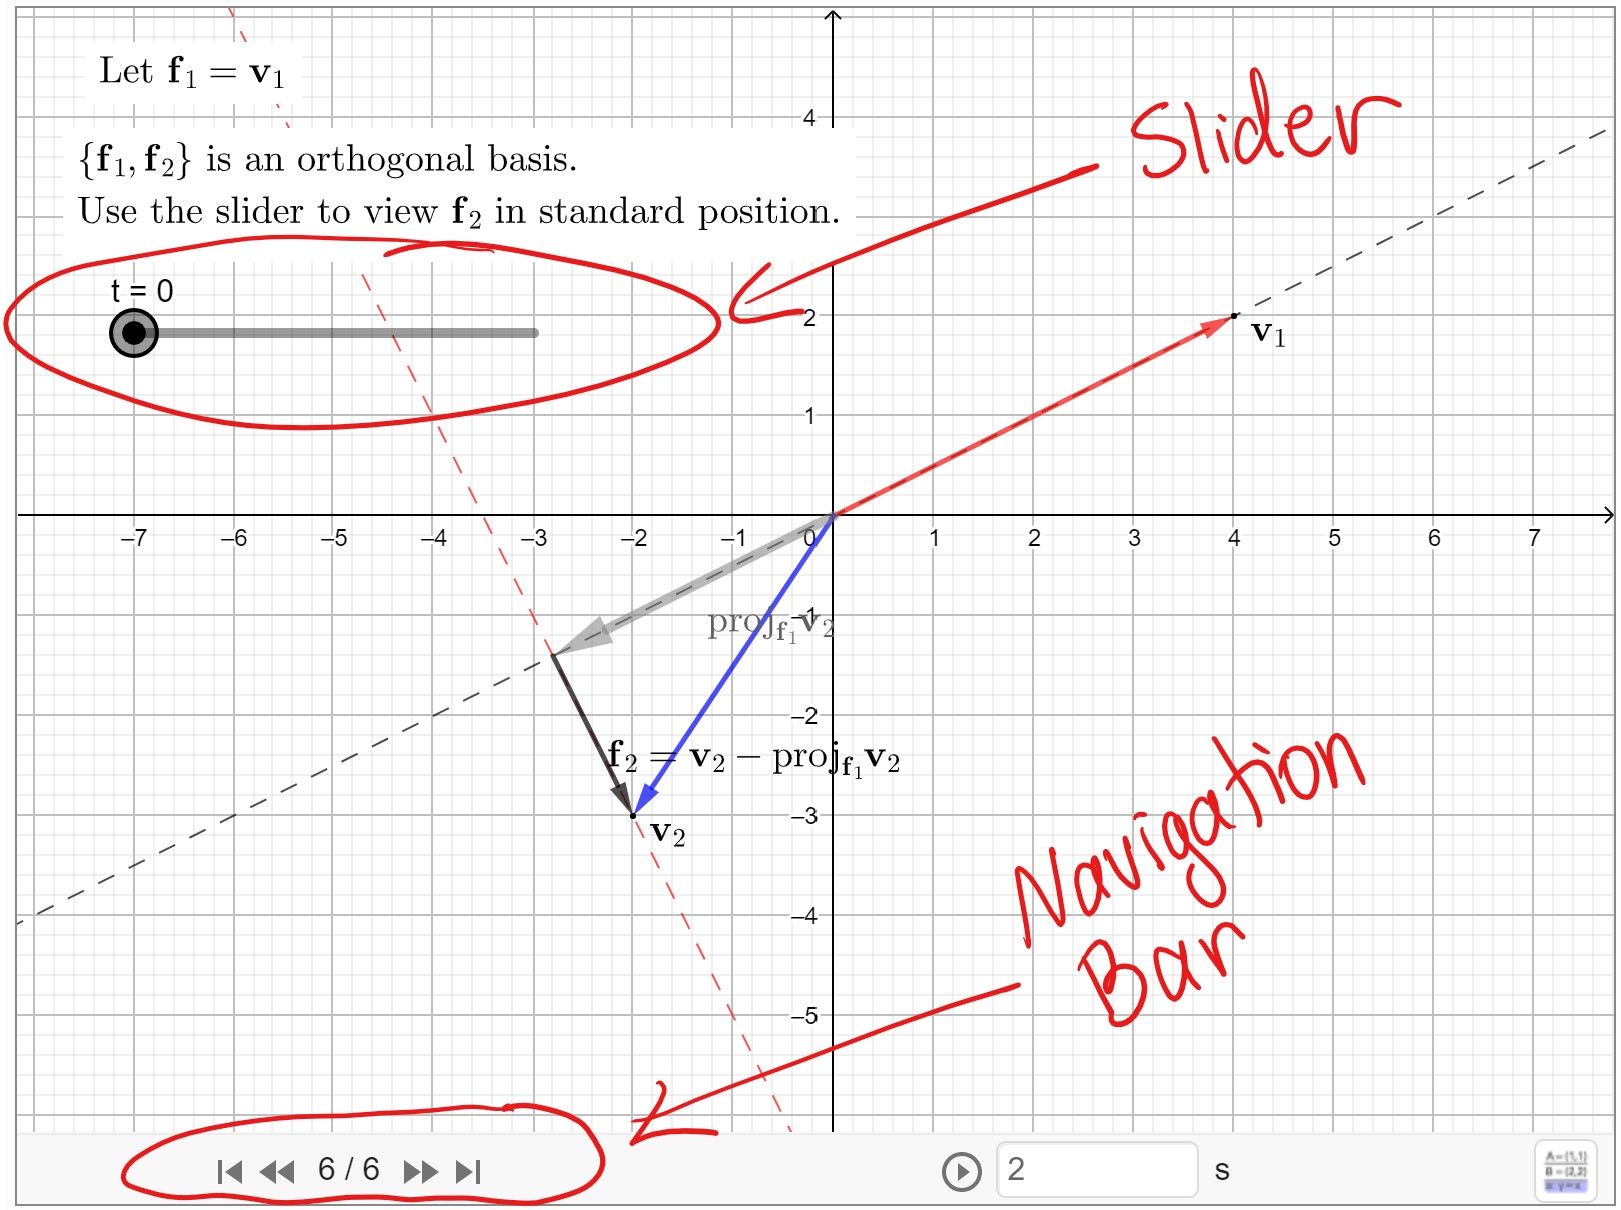
\includegraphics{GeoGebraScreenshot1.jpg}
\end{image}

\begin{center}
\geogebra{xtqppyav}{800}{600}
\end{center}
GeoGebra offers many more features.  Make sure to read the directions in each interactive!

\subsection*{Octave Cells}
Matrix calculations are easy to perform using Octave cells.  Octave exercises appear in the Additional Exercises section at the end of each chapter.  A few other sections also contain Octave exercises.%, indicated by the following:

To use Octave, go to the \href{https://sagecell.sagemath.org/}{Sage Math Cell Webpage}, copy the code below into the cell, select OCTAVE as the language, and press EVALUATE.

If you click the link to go to the \href{https://sagecell.sagemath.org/}{Sage Math Cell Webpage}, you will see the image below.  Notice the dropdown menu in the lower right-hand corner where you can select Octave as the language.  Try copying the following code into a cell to see how it works.

\begin{verbatim}
% Understanding matrix-vector multiplication as linear combinations of columns
A=[2 -1 3 2; 0 3 -2 1; -2 4 1 0];
x=[3;-1;4;1]; %semicolons at the end of a line suppress the output
x(1)*A(:,1)+x(2)*A(:,2)+x(3)*A(:,3)+x(4)*A(:,4)
A*x
\end{verbatim} 

\begin{image}
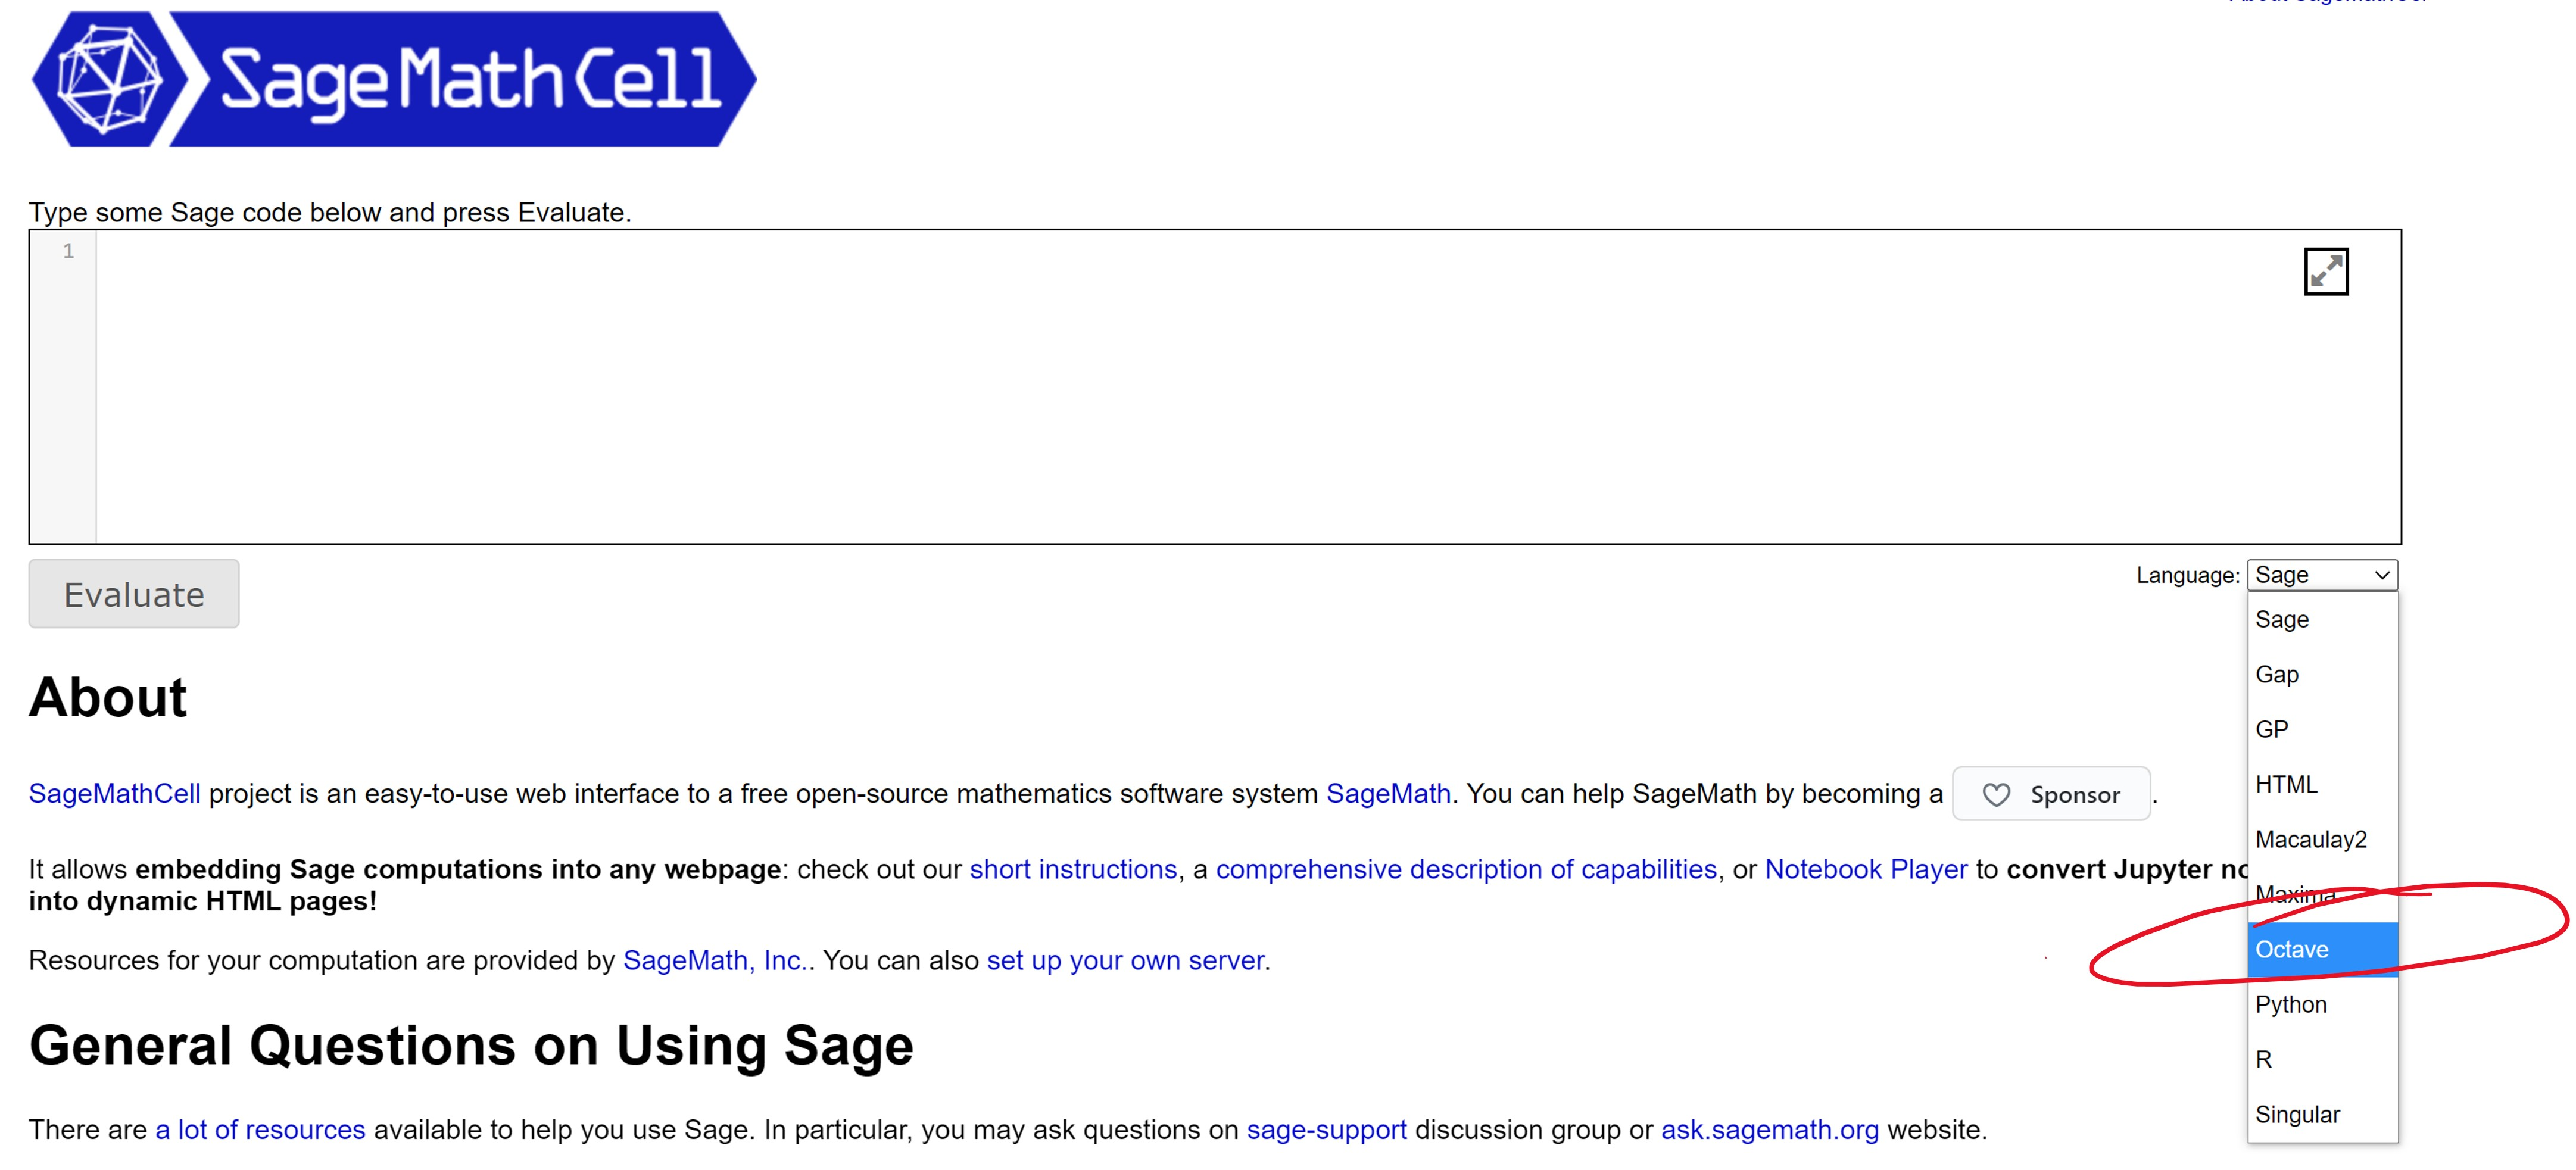
\includegraphics{SageCell.jpg}
\end{image}

Be sure to select Octave as the language or the code will yield an error when you press evaluate.

\subsection*{Saving your Work and Keeping Track of Progress}
One of the most common questions about XIMERA is, "Do I have to log in to use it?"  Here is what we recommend:
\begin{itemize}
\item If you don't care whether or not you keep your work, do NOT log in.  XIMERA gives full access to all users, regardless of log-in status.
\item If you want to keep track of your progress and your answers, then
\begin{itemize}
\item If you plan on using the same computer for all of your XIMERA work, the easiest thing to do is NOT log in.  Your answers will be saved automatically, and XIMERA will remember your progress.  WARNING: You will lose your work if you clear out your cookies.
\item If you plan to use multiple machines to do your XIMERA work, then you may want to log in, so that XIMERA knows who you are regardless of your computer.  WARNING: If you decide to start logging in, you have to continue to log in, otherwise XIMERA will think of you as multiple people.
\end{itemize}
\end{itemize}

Instructors may require that you submit a proof of completion.  This is easy to do. 
\begin{itemize}
    \item Go to the landing page for the course.
    \begin{image}
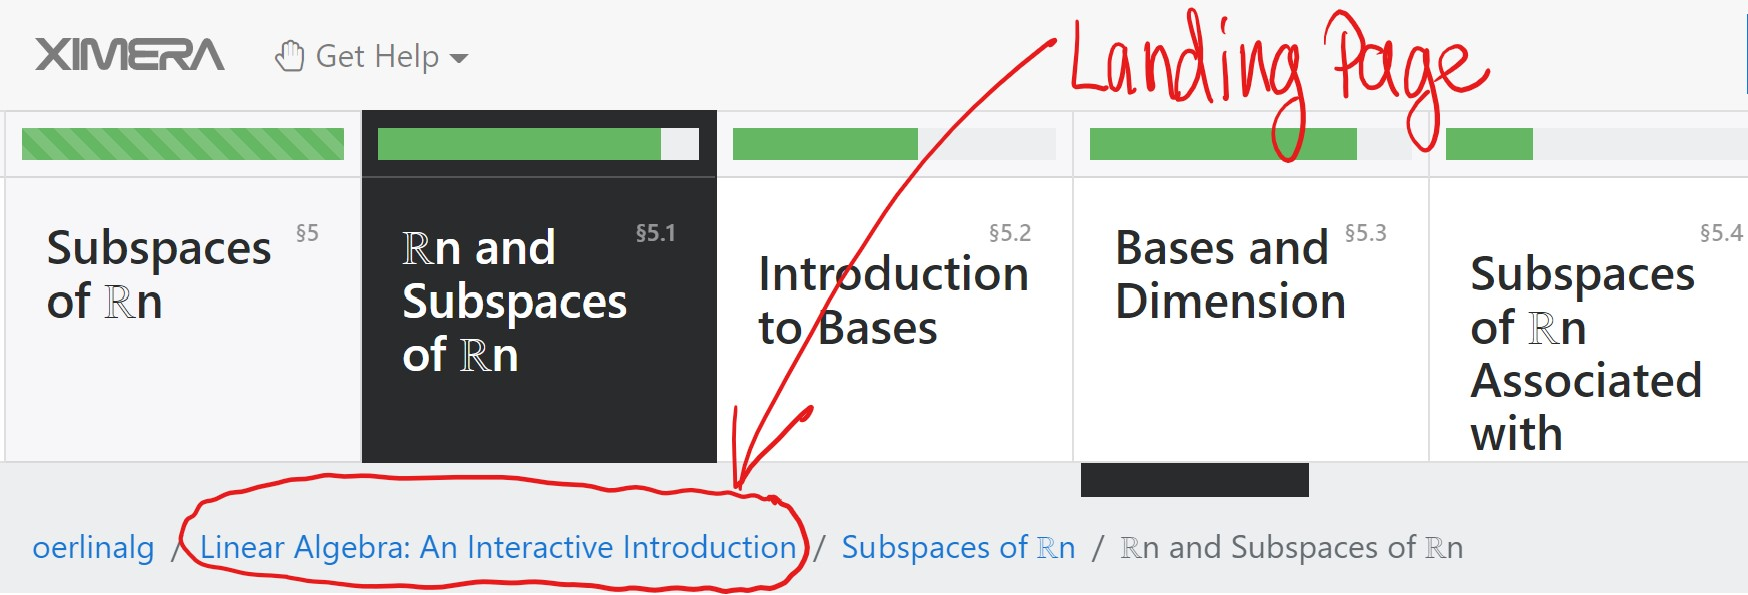
\includegraphics{ximeraScreenshot1.jpg}
\end{image}
\item Scroll to the bottom of the page and click on the Certificate button.
\begin{image}
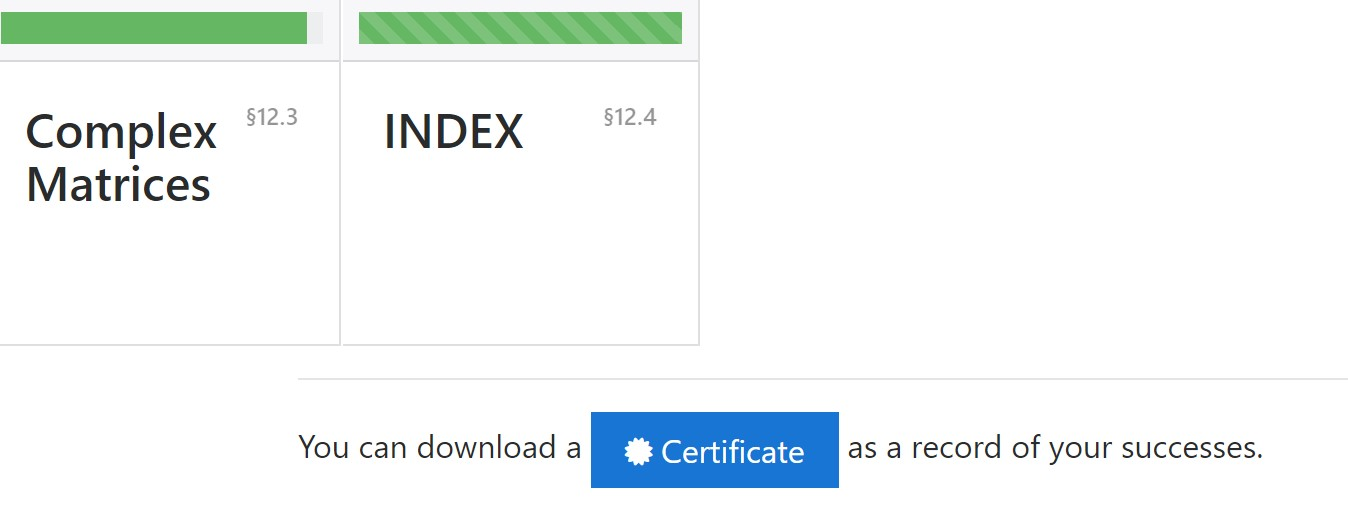
\includegraphics{ximeraScreenshot2.jpg}
\end{image}
\item
Your instructor may ask you to submit a screenshot of your completion summary.
\begin{image}
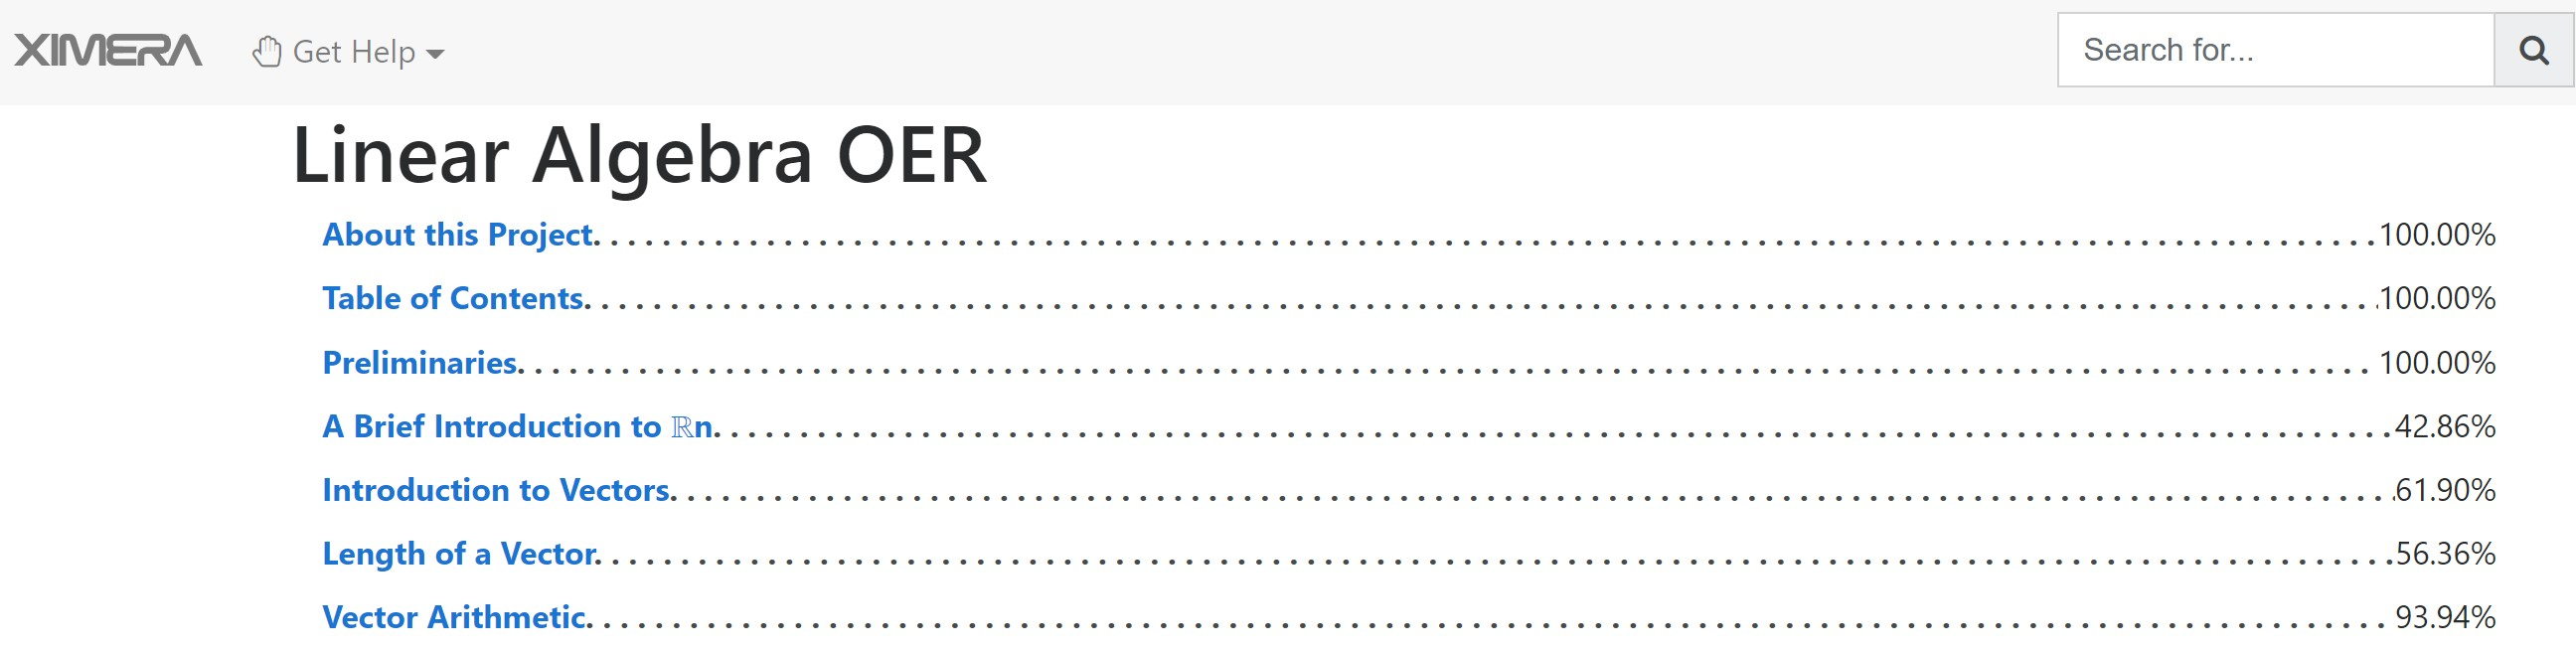
\includegraphics{ximeraScreenshot3.jpg}
\end{image}
\end{itemize}
\subsection*{Data Collection and Usage}
Event stream data from user interactions with the platform -- such as mouse clicks, and submitted answers -- are stored on a secure server at the Ohio State University.  There is no plaintext storage of passwords, and only encrypted protocols for authentication are used.  Anonymized event log is available to the authors of this text through secure access requiring a private key. (GPG is used for this.)   Event log data may be used for research purposes and to improve the product.
\end{document}
